\chapter{Fragments}
\label{FRAG}

\section{Introduction}
\label{FRAG:introduction}
What are \href{https://developer.android.com/guide/components/fragments.html}{Fragments}? To simply put they are \textit{reusable} components that can render user interface elements on the screen and run java code. However they are NOT activities and they are NOT containers such as linear layout.

You might ask that \texttt{LinearLayout} or any other layout is also a container and you can put all your interface in it as well. That is true indeed! But if you want to add say a specific form to 20 different activities in your app. You will have to create 20 separate layouts having pretty much the same repeating code. From a software engineering point of view repetitive code is very bad. If you want to change the color of the form then you need to modify it at 20 locations! On the contrary a fragment lets
you create a user interface \textit{only once} and then allow you to re-use this again and again without any limitations. 

In addition to being a container, a fragment also has its own simple life-cycle. You can think of a fragment as somewhat similar to a mini activity.

\begin{quote}
	\textit{``\textbf{Important:} Just like an activity, a fragment has a layout resource file and a java code file.''}
\end{quote}

As expected our custom fragment class will extend from the `\texttt{Fragment}' class which resides under `\texttt{android.app}' package. Historically fragments were not supported on some earlier android versions. In order to support them on lower android api you need to include support libraries and the corresponding package name such as `\texttt{android.support.v4.app}'.

\begin{quote}
	\textit{``\textbf{Important:} Fragments can not exist on their own independently. They must always reside inside a parent activity. There is no limit on the number of fragments that you can put inside an activity. \textbf{The fragments can not talk directly to each other.} We will see in detail in the future activities how we can go around this limitation.''}
\end{quote}

Apart from being reusable components, you can add, replace and delete any fragment from the activity at run-time. Something that is not easy to do with standard layouts. This means that you can design complex apps that adapt intelligently to the screen sizes. For example on a mobile device your app may run normally from activity to another activity. But on a tablet it may display two panes giving the illusion that two activities are running simultaneously on the same screen, as shown in figure below:

\begin{center}
	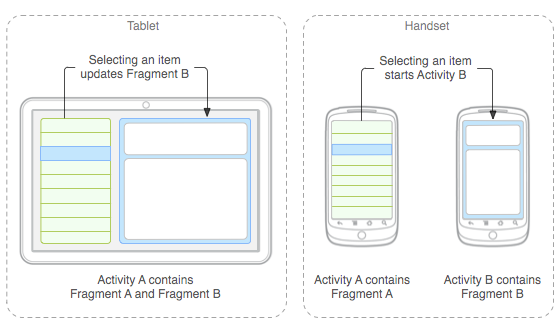
\includegraphics[scale=\FigureScale]{chapters/ch11/images/1}
\end{center}

Ok, enough theory. Let's start coding and see how fragments are actually made.

\section{Create New Project}
\label{FRAG:createProj}

Create a new project from scratch. Perform the following steps:
\begin{enumerate}
	\item Create a new project having name ``\texttt{Fragments}''
	\item Select minimum API 16 : Android 4.1 (Jelly Bean).
	\item Select ``\texttt{Empty Activity}''
	\item Accept default values for activity and click finish. \\
\end{enumerate}

\section{Fragment Creation}
\label{FRAG:fragmentCreation}
There are two ways to create a fragment. Either we can use the android studio wizard that guides the entire process step by step or we can create a fragment manually. For this activity let's choose the second option i.e creating it manually. \\

As it is mentioned earlier, a fragment is composed of a layout file and a java class. Let's create the layout first. The process is very similar to that of creating an activity layout. In the project panel on the left, right-click ``\texttt{layout}'' group, then ``\texttt{New}'' and then select ``Layout Resource File''. Give the name ``\texttt{green\_fragment.xml}'':

\begin{center}
	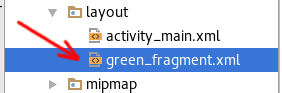
\includegraphics[scale=\SourceCodeScale]{chapters/ch11/images/2}
\end{center}

Open up ``\texttt{green\_fragment.xml}'' and go to design view. It is an empty layout. Add following user interface elements and also change the background to green. For this activity we are using pure green color \texttt{\#00ff00} but you are free to use any green tint:

\begin{center}
	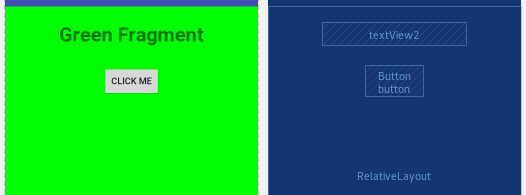
\includegraphics[scale=\FigureScale]{chapters/ch11/images/3}
\end{center}

Alright, our layout is looking pretty awesome. Now er need to create the corresponding java file. In the project panel, create a new java file in the same directory as \texttt{MainActivity.java}. Right click on the package group, select ``New $\rightarrow$ Java class'', name it ``\texttt{GreenFragment}'':

\begin{center}
	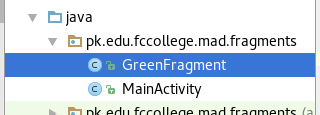
\includegraphics[scale=\SourceCodeScale]{chapters/ch11/images/4}
\end{center}

Open up \texttt{GreenFragment.java} file. Extend \texttt{GreenFragment} class from the ``\href{https://developer.android.com/guide/components/fragments.html}{\texttt{Fragment}}'' class. If you have included support libraries to your project then android studio will automatically include ``\texttt{android.support.v4.app}'' package. If not then you need to do it manually. Note that if android studio gives errors related to this support package then you can change the import statement (line 3 below) to ``\texttt{import android.app.Fragment}'':

\begin{center}
	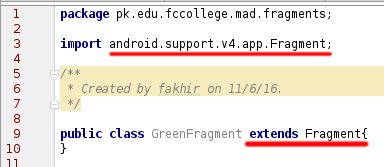
\includegraphics[scale=\SourceCodeScale]{chapters/ch11/images/5}
\end{center}

Now add an empty no argument constructor. Override a method named ``\texttt{onCreateView}''. The \texttt{onCreateView} is a fragment lifecycle method that gets called when the fragment is about to display its user interface. You can view fragment lifecycle diagram by clicking \href{https://developer.android.com/guide/components/fragments.html#Lifecycle}{here} and \href{https://developer.android.com/images/fragment_lifecycle.png}{here}. As compared to an activity the fragment lifecycle is simpler and linear.

\begin{center}
	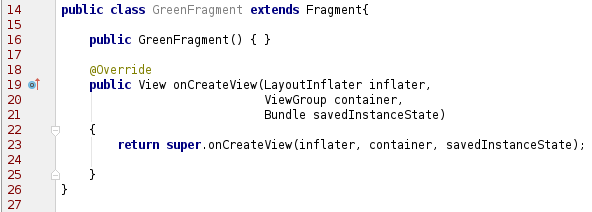
\includegraphics[scale=\SourceCodeScale]{chapters/ch11/images/6}
\end{center}

Line by line code analysis:

\begin{itemize}
	\item \textit{Line 19 to 21:} If you look at the fragment lifecycle methods, \texttt{onCreateView} method is called when the fragment is about to present itself on the screen. It takes the following three parameters:
	\begin{itemize}
		\item \textit{\textbf{inflater:}} The \texttt{LayoutInflater} object that can be used to inflate any views in the fragment.
		
		\item \textit{\textbf{container:}} If this is not null then it act as a parent of the fragment to which the fragment UI will be attached to. Ignore this parameter for now.
		
		\item \textit{\textbf{savedInstanceState:}} If it's not null then it may contain useful data/information for the current fragment to use. Ignore this parameter for now.
	\end{itemize}
	
	\item \textit{Line 23:} The code is returning default layout. We will create our own and return that, just like we did with the array adapter.
\end{itemize}

Since this method is called as soon as fragment is about to display the layout on the screen, we need to create a view that contains our layout and then finally return it (Looking suspiciously familiar with the custom \texttt{ArrayAdapter}'s ``\texttt{getView}'' method, isn't it?). Delete line 23 from above code and replace it with the following code:

\begin{center}
	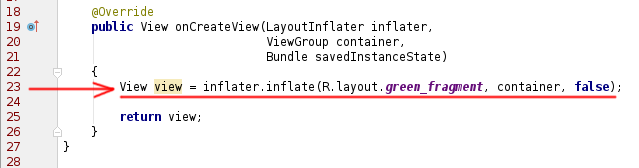
\includegraphics[scale=\SourceCodeScale]{chapters/ch11/images/7}
\end{center}

If you look at line 23 in the above listed code, you will notice that the first parameter is the layout resource file. Second is the parent container. Third is set to false, which means that we don't want to attach this view to the parent again, since we
are already returning it. In line 25 we are returning the newly created view object for our fragment. \\

Let's add some interactivity to the fragment button. First go to the \texttt{green\_fragment.xml} layout file and change the button id to ``\texttt{greenFragBtn}''. Now open up \texttt{GreenFragment.java}. In
the \texttt{onCreateView} method, we first get a reference to the desired button that resides inside the view and then attach an on click listener to it. Following code should look very familiar (\textit{lines 27-36}):

\begin{center}
	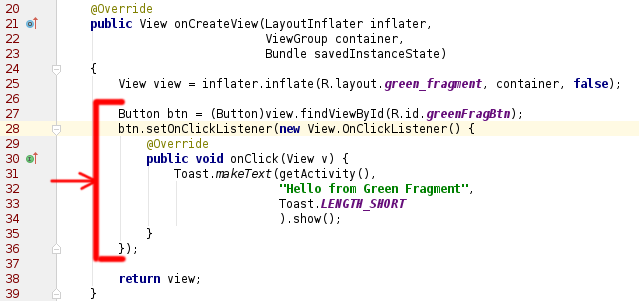
\includegraphics[scale=\SourceCodeScale]{chapters/ch11/images/8}
\end{center}

Our green fragment is pretty much complete. If you like you can add extra controls on its layout to make it a bit more complex but that is optional for this activity. \\

Recall that a fragment can not exist on its own, it needs to be attached to a parent activity. There are two ways to do that, let's look at these one by one.

\section{Attaching Through Layout Resource}
Open up \texttt{acvitity\_main.xml} and delete the default ``Hello World'' text view. This should result in an empty layout. Now switch to the design mode. In the palette panel on the left find fragment under the ``Layouts'' group:

\begin{center}
	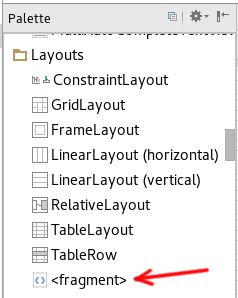
\includegraphics[scale=\SourceCodeScale]{chapters/ch11/images/9}
\end{center}

Drag a \texttt{<fragment>} and drop it onto the empty layout. A dialog box appears asking you what type of fragment do you want to add. Select \texttt{GreenFragment} from the list. Hit OK to finalize the selection:

\begin{center}
	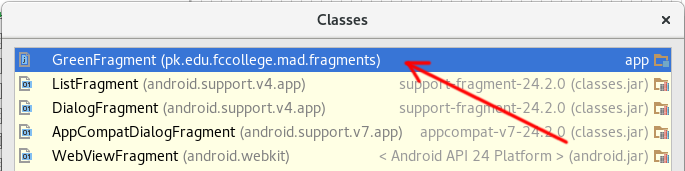
\includegraphics[scale=\SourceCodeScale]{chapters/ch11/images/10}
\end{center}

We just gave the java file. Now we need to specify the corresponding layout file. If not already, open up \texttt{activity\_main.xml} in design mode. You may see the following rendering errors. Click on ``\texttt{@layout/green\_fragment.xml}'' (marked with red):

\begin{center}
	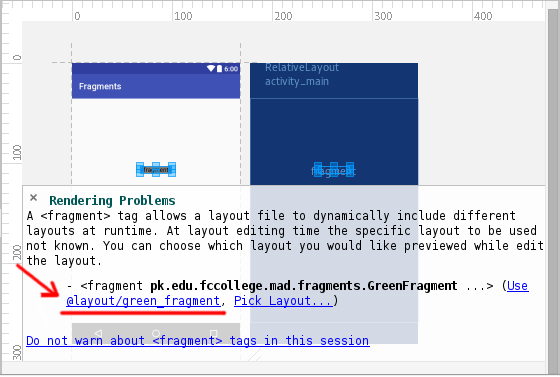
\includegraphics[scale=\FigureScale]{chapters/ch11/images/11}
\end{center}

After the design view refreshes you should see the green fragment layout properly embedded inside the \texttt{<fragment>} container. You can resize the fragment container to anything you like (for this activity it's layout width and height have been set to $300dp$ and $250dp$ respectively):

\begin{center}
	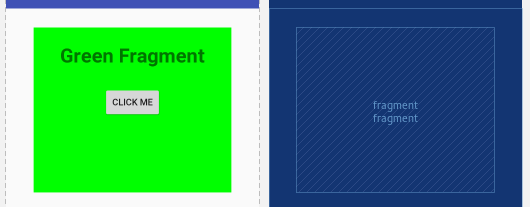
\includegraphics[scale=\FigureScale]{chapters/ch11/images/12}
\end{center}

Run the app on a device and you will see following output. Click the button and you should see a toast being displayed:

\begin{center}
	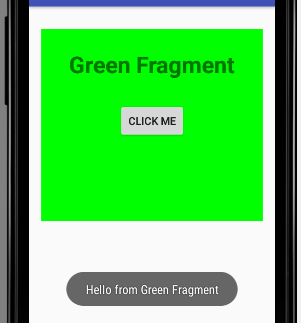
\includegraphics[scale=\FigureScale]{chapters/ch11/images/13}
\end{center}

You can add this fragment to as many activities as you wish. If you want to change the color from green to blue then you only need to change it once and it will automatically update everywhere!

\section{Attaching Through Java Code}
\label{FRAG:attachingThroughJava}
To add fragments through code we will need something called a ``\href{https://developer.android.com/guide/components/fragments.html#Transactions}{\textit{Fragment Manager}}''. A fragment manager is responsible for adding, deleting, replacing, suspending fragment dynamically at run-time. Once you have a reference to the fragment manager, you begin a ``\textit{transaction}''. A transaction is just a series of ``\texttt{add}'', ``\texttt{delete}'', ``\texttt{replace}'' commands. Once you've written all the commands, you finally need to finish the transaction by committing it using the ``\texttt{commit}'' method. \\

Go to \texttt{activity\_main.xml} and delete the fragment container. You should end up with an empty layout similar to the following:

\begin{center}
	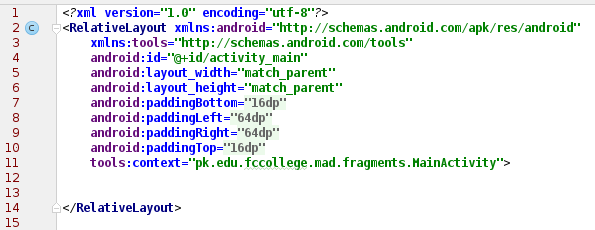
\includegraphics[scale=\SourceCodeScale]{chapters/ch11/images/14}
\end{center}

You can add a fragment inside any type of ``\texttt{ViewGroup}'' container. For our purposes we will use a ``\texttt{FrameLayout}'' (you are free to use linear or relative layout etc). A frame layout can contain only one element at a time. While inside \texttt{activity\_main} layout text mode, add a frame layout element. Set its
width to ``$300dp$'' and its height to say ``$250dp$'' (\textit{lines 13 to 20}):

\begin{center}
	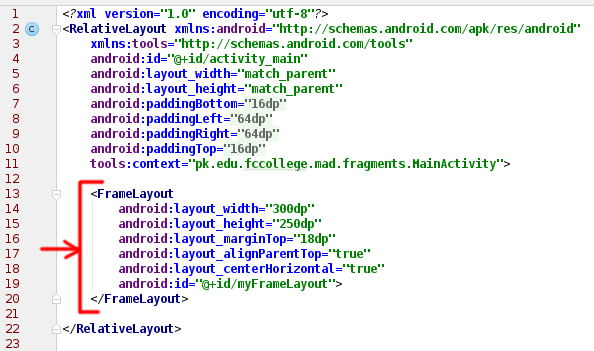
\includegraphics[scale=\SourceCodeScale]{chapters/ch11/images/15}
\end{center}

\textbf{Extremely important:} Don't forget to set its id as done in line 19 above. We need the \texttt{id} to refer to this container from java code. \\

Great! Our layout file is finished. Now open up \texttt{MainActivity.java}. Inside the \texttt{onCreate} method, write the following code (\textit{lines 15 to 20}):

\begin{center}
	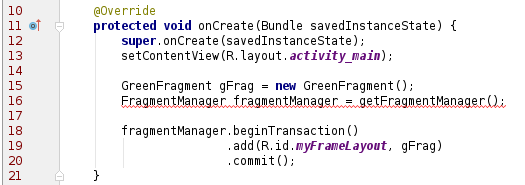
\includegraphics[scale=\SourceCodeScale]{chapters/ch11/images/16}
\end{center}

Line by line explanation of the above code:

\begin{itemize}
	\item \textit{Line 15:} Create a new instance of the fragment that we want to use.
	\item \textit{Line 16:} Get an instance of the fragment manager. Fragment manager is responsible for adding, replacing, removing fragments dynamically. Note that you may get ``support library'' related errors. They are very easy to fix as explained in the `important tip' below.
	\item \textit{Line 18 to 20:} This is one single complex statement. Let's break it down bit by bit:
	\begin{itemize}
		\item \textit{Line 18:} Before doing anything you need to begin a transaction.
		
		\item \textit{Line 19:} Here we are adding a fragment to the container. The \texttt{add} method accepts two parameters. First is the \texttt{id} of the container we want our fragment to reside inside of. Second is the actual fragment object.
		\item \textit{Line 20:} Finally to make the changes take place you need to commit the transaction.
	\end{itemize}
\end{itemize}

\begin{quote}
	\textit{``\textbf{Important:} \underline{In case if} android studio gives an error while adding fragment manager (just like above) it means that you do not have proper support libraries installed. The solution to this is very simple. Go to the top of \texttt{MainActivity.java} file and change the import package from \texttt{android.support.v4.app.FragmentManager} to \texttt{android.app.FragmentManager} as shown below (line 3):}

	\begin{center}
		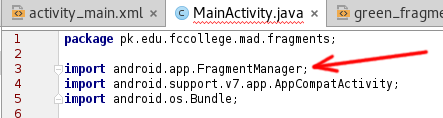
\includegraphics[scale=\SourceCodeScale]{chapters/ch11/images/17}
	\end{center}
	
	\textit{You also need to open up \texttt{GreenFragment.java} and change the fragment package from \texttt{android.support.v4.app.Fragment} to \texttt{android.app.Fragment} as shown (line 4):}
	
	\begin{center}
		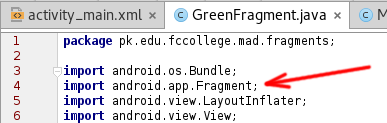
\includegraphics[scale=\SourceCodeScale]{chapters/ch11/images/18}
	\end{center}
	
	\textit{Following these simple steps should resolve any support related errors.''}
\end{quote}

Run the app and you should see the green fragment properly rendered on the screen and showing a toast on button click as expected.

\section{Exercise 1}

Make a red fragment (as shown below). Try to load this one instead of the green one in the main activity. Whenever the button is clicked an appropriate toast should be displayed such as \textit{``Hello from Red Fragment''}:
	
\begin{center}
	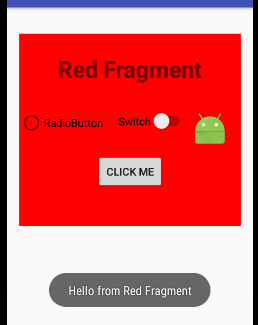
\includegraphics[scale=\FigureScale]{chapters/ch11/images/19}
\end{center}
	
\section{Exercise 2}
\label{FRAG:exercise2}
Create a layout for the main activity to support \textit{landscape} mode. Add both red and green fragments side by side on this layout. Run the app on a device and switch to portrait mode. You should see the following output:

\begin{center}
	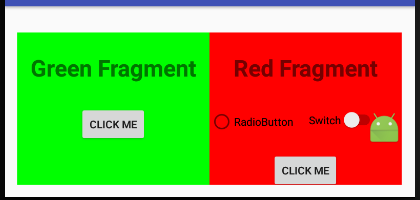
\includegraphics[scale=\FigureScale]{chapters/ch11/images/20}
\end{center}

Note that the app MUST work correctly in both portrait and landscape modes. In portrait mode it shows just one fragment, in landscape mode it renders two fragments as shown in the figure above. \\

\textbf{Hint:} Note that in portrait mode there is only one fragment container whereas in landscape mode there are two. You need to be careful assigning the \texttt{id}s to the containers. Also you need to check whether the phone is in portrait mode or landscape mode and then write your logic accordingly.

\section{Replacing Fragments}
Sometimes we need to replace one fragment with another at run-time. Let's see how to do that. It's actually pretty simple. Open up \texttt{activity\_main.xml} (portrait mode). Under the already existing frame layout container add a button having an id of ``\texttt{myToggleBtn}'' and label ``\textit{Toggle Frames}'':

\begin{center}
	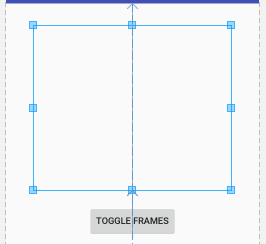
\includegraphics[scale=\FigureScale]{chapters/ch11/images/21}
\end{center}

Attach an event listener named \texttt{onToggleBtnCLick} to this button and add following code, all of this should look very familiar (notice the \texttt{toggle} variable defined in line 32):

\begin{center}
	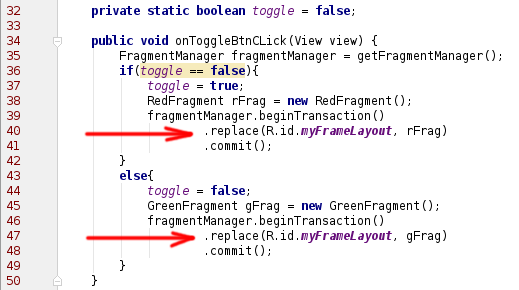
\includegraphics[scale=\SourceCodeScale]{chapters/ch11/images/22}
\end{center}

\begin{quote}
	\textit{``\underline{\textbf{Extremely important:}} Note closely lines 43 and 47. We are calling the \texttt{replace} method instead of \texttt{add}. If you call \texttt{add} when you wanted to replace a fragment then you may see weird results on the screen, the app may even crash!''}
\end{quote}

Run the app and enjoy toggling some fragments !

\section{Communication Between Fragments}

Before moving on, we need to create simple fragments. Do the following exercise before going any further.

\subsection{Exercise 3}
Close any currently open projects and create a new project following the steps mentioned in section \ref{FRAG:createProj}, name this project \texttt{Fragments2}. Create and embed two fragments inside the main activity (add the fragments through java code using fragment manager as illustrated in section \ref{FRAG:attachingThroughJava}). Make sure it is running without errors on the emulator and the green buttons display appropriate toasts (also see the rules given below):

\begin{center}
	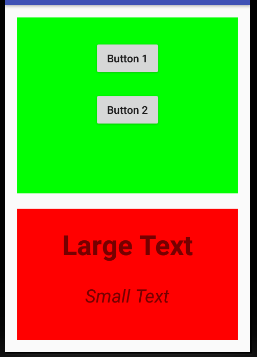
\includegraphics[scale=\FigureScale]{chapters/ch11/images/23}
\end{center}

Following rules MUST be followed:
\begin{itemize}
	\item Main Activity:
	\begin{itemize}
		\item Contains two frame layouts having \texttt{id}s: ``\texttt{greenFragFrame}'' and ``\texttt{redFragFrame}''.
	\end{itemize}

	\item Green Fragment:
	\begin{itemize}
		\item Layout file: ``\texttt{green\_frag.xml}''
		\begin{itemize}
			\item Button 1 id: ``\texttt{greenFrag\_btn1}''
			\item Button 2 id: ``\texttt{greenFrag\_btn2}''
		\end{itemize}
		
		\item Java class name: ``\texttt{GreenFrag}''
	\end{itemize}
	
	\item Red Fragment:
		\begin{itemize}
			\item Layout file: ``\texttt{red\_frag.xml}''
			\begin{itemize}
				\item Text View 1 id: ``\texttt{red\_textTop}''
				\item Text View 2 id: ``\texttt{red\_textBottom}''
			\end{itemize}
			
			\item Java class name: ``\texttt{RedFrag}''
		\end{itemize}
\end{itemize}

\subsection{Communication Pathways}
\label{FRAG:communicationPathways}

Fragments are made for reusability. That's why the fragments SHOULD NEVER communicate with each other directly. This would hinder their modularity and reusability. In case if they need to send messages they do it via the parent activity within which these fragments are contained. Following figure shows communication pathways between fragments and parent activity:

\begin{center}
	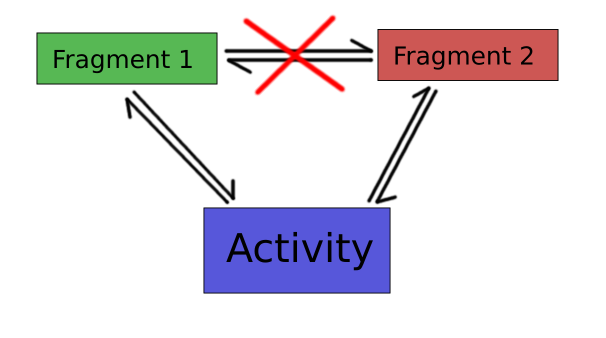
\includegraphics[scale=0.3]{chapters/ch11/images/24}
\end{center}

For this task our goal is very simple. The top button in the green fragment will set the top text view of the red fragment. Similarly the bottom button in the green fragment will change the bottom text view of the red fragment. To simplify the green fragment will send messages to the main activity and in turn the main activity will send messages to the red fragment. Let's see how these communications take place.

\subsection{From Fragment to Activity}
\label{FRAG:fromFragmentToActivity}

In order to send messages from a fragment to the parent activity we need to define an interface and then implement the parent activity using this interface. By sending messages to the activity we mean calling activity's methods from the fragment. \\

Create a new interface named ``\texttt{Communicate}'' in the same folder as \texttt{MainActivity.java}. You can name the interface anything you like. It can contain any type of method imaginable. We are adding the following two because we plan to change the text views of the red fragment:

\begin{center}
	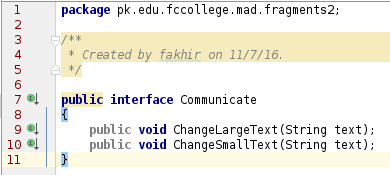
\includegraphics[scale=\SourceCodeScale]{chapters/ch11/images/25}
\end{center}

Calling parent activity's method from a fragment is the same as sending a message FROM the fragment TO the parent activity. Generally speaking this interface will contain all methods of the parent activity that we want to call from a fragment. 

\begin{quote}
	\textit{``\textbf{Important:} If you want to communicate (send message) FROM a fragment TO an activity you will define methods in this interface.''}
\end{quote}


Open up \texttt{MainActivity.java} and implement it with the \texttt{Communicate} interface:

\begin{center}
	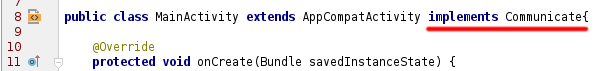
\includegraphics[scale=\SourceCodeScale]{chapters/ch11/images/26}
\end{center}

Also implement interface methods. Override the following methods inside \texttt{MainActivity} class. For now we are simply displaying toasts in each of these. We will modify these methods later:

\begin{center}
	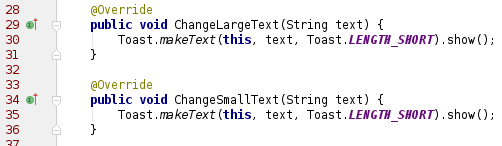
\includegraphics[scale=\SourceCodeScale]{chapters/ch11/images/27}
\end{center}

Open up \texttt{GreenFrag.java} and add the following variables near the top of the class:

\begin{center}
	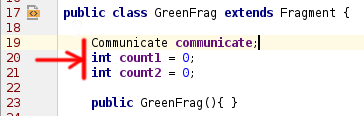
\includegraphics[scale=\SourceCodeScale]{chapters/ch11/images/28}
\end{center}

Line 19 defines a variable of type \texttt{Communicate}. Remember that \texttt{MainActivity} implemented \texttt{Communicate} interface? So this variable will hold the reference to the parent activity i.e the \texttt{MainActivity}. Lines 20 and 21 define two integer counters that will be incremented on each button click in the green fragment. \\

Next step is to save a reference of the parent activity. There is a fragment lifecycle method called ``\href{https://developer.android.com/reference/android/app/Fragment.html#onAttach(android.app.Activity)}{\texttt{onAttach}}'' that gets called as soon as the fragment is added or attached to a parent container. The parameter \texttt{context} is the reference to the parent activity which is actually \texttt{MainActivity}. We save this in the \texttt{communicate} variable for future use. Why communicate variable? because remember that we implemented \texttt{MainActivity} from \texttt{Communicate} interface so \texttt{MainActivity} is of type \texttt{Communicate}: 

\begin{center}
	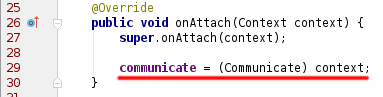
\includegraphics[scale=\SourceCodeScale]{chapters/ch11/images/29}
\end{center}

Finally inside the \texttt{onCreateView} create and return fragment view just like we did earlier. Additionally we are attaching event listeners to both the green fragment buttons. The following code should look very familiar.

\begin{center}
	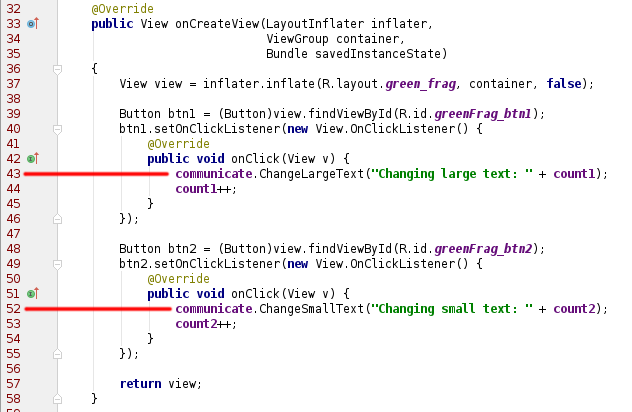
\includegraphics[scale=\SourceCodeScale]{chapters/ch11/images/30}
\end{center}

The lines to note are 43 and 52. When any green fragment button is clicked we are calling corresponding methods of the \texttt{MainActivity}. The counters are also incremented on each button click. \\

Run the app on a device and you should see toasts when ever you click any green fragment button.

\subsection{From Activity to Fragment}
\label{FRAG:fromActivityToFragment}

Calling fragment's methods FROM activity or in other words sending messages FROM activity TO fragment is rather very simple. Just crate fragment object in the activity class and call its public methods, that's all! 

Open up \texttt{RedFrag.java}. We need to save the references to both the text views. Create two class member variables near the top (\textit{lines 16 and 17}):

\begin{center}
	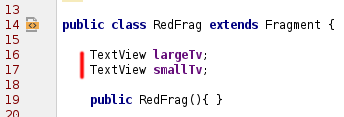
\includegraphics[scale=\SourceCodeScale]{chapters/ch11/images/31}
\end{center}

In the \texttt{onCreateView} method find and save references to these text views (\textit{lines 28 and 29}):

\begin{center}
	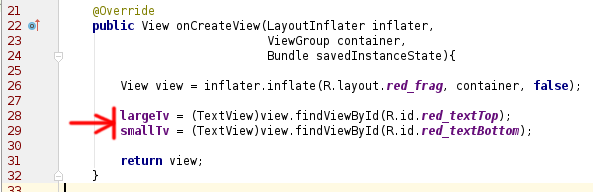
\includegraphics[scale=\SourceCodeScale]{chapters/ch11/images/32}
\end{center}

And add the following public methods for setting each of the text view:

\begin{center}
	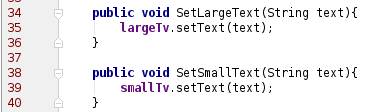
\includegraphics[scale=\SourceCodeScale]{chapters/ch11/images/33}
\end{center}

We are almost done. We just need to make minor modifications to \texttt{MainActivity} class. Open up \texttt{MainActivity.java}. First thing is to make the fragment objects as member variables:

\begin{center}
	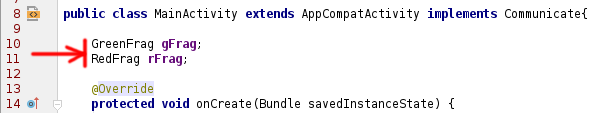
\includegraphics[scale=\SourceCodeScale]{chapters/ch11/images/34}
\end{center}

Also make sure that you are using these member variables within the \texttt{onCreate} method and NOT creating local variables for fragment objects. Finally go to the change text methods and replace the toasts with the following code that actually sets the text for the red fragment (\texttt{lines 33 and 38}):

\begin{center}
	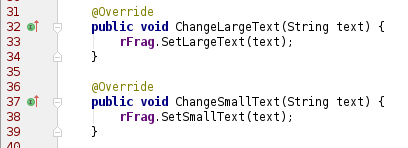
\includegraphics[scale=\SourceCodeScale]{chapters/ch11/images/35}
\end{center}

Run the app on a device. When ever you click any green fragment button the corresponding red fragment text view should update:

\begin{center}
	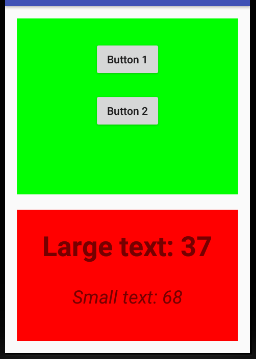
\includegraphics[scale=\FigureScale]{chapters/ch11/images/36}
\end{center}

You can read more about fragment communication \href{https://developer.android.com/training/basics/fragments/communicating.html}{here}.

\subsubsection{Exercise}
Open up \texttt{GreenFrag.java}. Suppose that you replace line 18 with \texttt{MainActivity myActivity}:

\begin{center}
	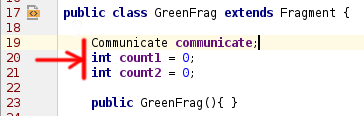
\includegraphics[scale=\SourceCodeScale]{chapters/ch11/images/28}
\end{center}

Now you can call all the public methods of \texttt{MainActivity} class. So inside the green fragment button's click listeners instead of:

\texttt{communicate.ChangeLargeText("Large text: " + count1);}

We could simply call the \texttt{MainActivity} object and that WILL work OK in this case:

\texttt{myActivity.ChangeLargeText("Large text: " + count1);} \\

The question is what is the purpose of painfully creating the \texttt{Communicate} interface? Why cant we just use \texttt{MainActivity} object and call its public member functions in all cases?


\section{Important Exercise}
Create a simple app that displays information about a list of employees. You can hardcode the list of employees if you want.
\begin{itemize}
	\item When the app is run in portrait mode it should display employee names in a list. As soon as the user taps on a list item it should launch a separate activity listing employee details.
	
	\item When the app is run in landscape mode then it should display the list view and the details panel side by side on a single screen. Clicking on any list view item should properly update the employee information in the other panel.
\end{itemize}

\textbf{Requirement:} You MUST use fragments. There should be no code/xml duplication.

\begin{center}
	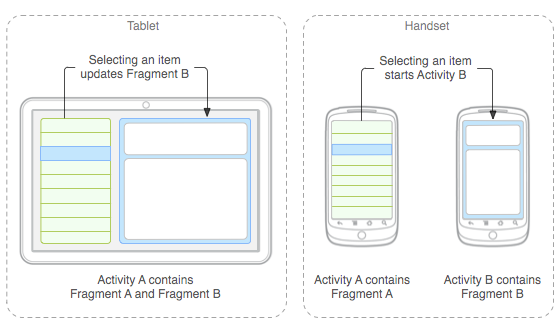
\includegraphics[scale=\FigureScale]{chapters/ch11/images/1}
\end{center}
